Tässä kappaleessa käsitellään uutta kaatosysteemiä, jonka avulla pyritään ratkaisemaan edellisessä kappaleessa käsiteltyjä ongelmia. Kaatosysteemin käsittely sisältää sekä logiikan että robottikoodin ja näiden kahden rajapinnan.

Uudessa kaatosysteemissä käytetään ikään kuin takaisinkytkentänä vaakaa, jolloin saadaan tietoon mukissa oleva massa kaadon aikana. Tässä vaakana on käytetty kappaleessa \ref{ch:drinkkirobotti_5.0} esiteltyä pullonvaihtopisteellä käytettyä vaakaa, mutta mikä tahansa samalla toimintaperiaatteella toimiva painoanturi kävisi tähän tarkoitukseen. Vaa'an NodeMCU:lta voidaan pyytää painoanturin osoittamaa massaa tietyllä merkkijonolla. Vaaka voidaan myös taarata toisella siihen tarkoitetulla merkkijonolla. Robotin logiikkaan on tehty oma ScaleCommunication-taso, joka ottaa yhteyden vaakaan. Sen metodeilla getWeight() ja Tare() pystyy suoraan käyttämään vaakaa logiikasta.

% TODO Lisää tietoa LogicLayerin toiminnasta tähän tai kpl 2.1?

Logiikkakerros kutsuu logiikan funktiota PourBottle, joka käsittelee kaatoa yksittäisestä pullosta. Nyt uutena logiikkaan on toteutettu funktio HandlePour. Tämä kutsuu vaakaa ja käskee robottia lopettamaan kaadon, kun vaa'an lukema on tarpeeksi suuri.

\begin{figure}[h]
\begin{center}
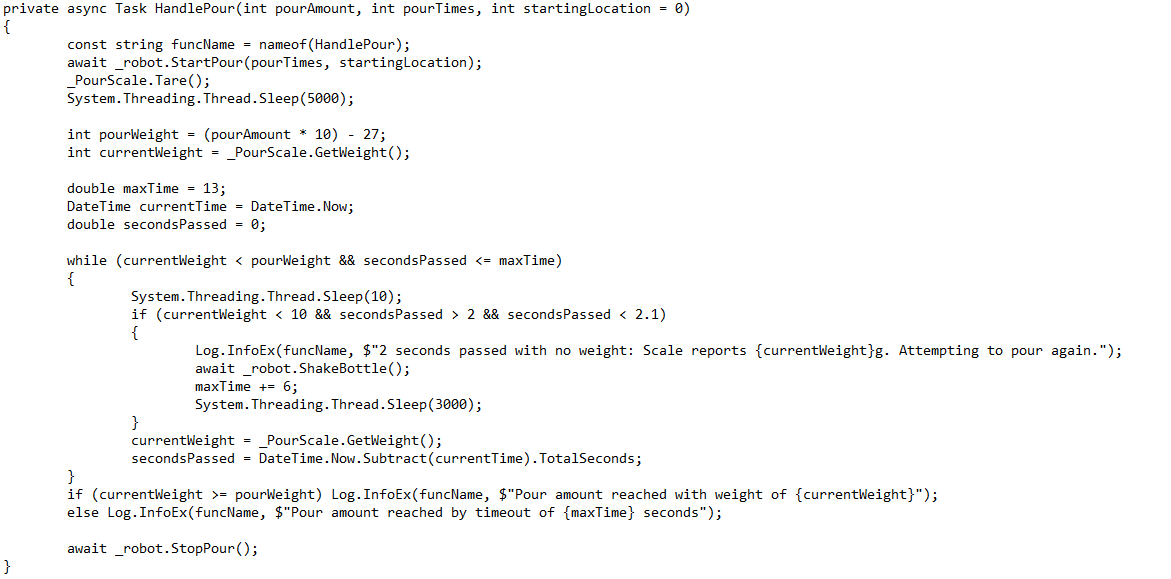
\includegraphics[scale=0.6]{img/HandlePour.png}
\end{center}
\caption{HandlePour-funktio}
\label{fig:HandlePour}
\end{figure}

HandlePour kutsuu ensin RobotCellLayerin funktiota StartPour. RobotCellLayer vastaa robotin kanssa kommunikoinnista. StartPour kutsuu robotin jobia, joka on tällä hetkellä nimellä NEWPOUR.

\begin{figure}[h]
\begin{center}
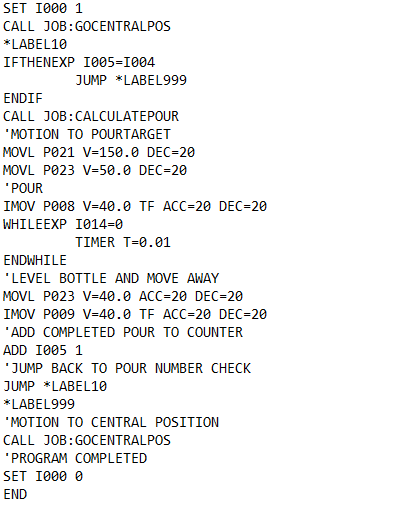
\includegraphics[scale=0.8]{img/NEWPOUR.png}
\end{center}
\caption{NEWPOUR-robottijobi}
\label{fig:NEWPOUR}
\end{figure}
%\newpage

NEWPOUR-job on robotin liikkeiltään hyvin samantapainen kuin kappaleessa \ref{ch:vanha_kaato} esitetty POURDRINKS. Aluksi se määrittää kaadettavan mukin sijainnin CALCULATEPOUR-jobilla. Sitten robottia käsketään siirtymään kaatopisteelle ja robotti kallistaa pulloa aloittaen kaadon. Uutta on kuitenkin se, että robotti jää while-loopin ansiosta odottamaan, että muuttuja I014 on 0. I014 on nimetty robotissa nimellä "pour ready signal".

HandlePour-funktio laskee halutun painon kertomalla halutun nesteen tilavuuden, joka on senttilitroina, kymmenellä, jolloin saadaan haluttu massa grammoina. Tästä vähennetään vielä vakio 27. Tämä vakio on määritetty testaamalla ja se kuvaa sitä viivettä, joka kestää siitä kun vaaka tunnistaa massan olevan sopiva, siihen kun nestettä ei enää tule ollenkaan mukiin.

Funktiossa on myös määritelty vakio maxTime, joka on 13 sekuntia. Tämä vakio on määritetty sen perusteella, että kappaleessa \ref{ch:vanha_kaato} esitellyn kaatoajan funktion mukaan saadaan 13 sekunnin kaadolla n. 25 senttilitraa juomaa. Drinkkirobotin tarjoilussa käyttämät lasit ovat tavallisesti hieman yli 25 senttilitraa tilavuudeltaan. Tätä maxTime-vakiota käytetään siihen, ettei mahdollisessa vaa'an virhetilanteessa juomaa kaadeta siten, että se läikkyisi lasista yli.

Fuktiossa on while-looppi, joka odottaa joka iteraatiolla kymmenen millisekuntia, kysyy uutta vaa'an havaitsemaa massaa, ja sen jälkeen tarkistaa onko havaittu massa yhä pienempi kuin haluttu massa. Samalla looppi tarkistaa, ettei kaato ole kestänyt yli maxTime-vakiossa määriteltyä aikaa. Kun while-loopista on tultu ulos, niin tulostetaan konsoliin tieto saavutetusta massasta tai mahdollisesti ajasta ja kutsutaan RobotCellLayerin funktiota StopPour.

StopPour-funktion tehtävänä on ainoastaan muuttaa robotin muuttuja I014, eli "pour ready signal" arvoon yksi. Tällöin robotin jobi tulee omasta while-loopistaan ulos, jolloin robotti suoristaa pullon ja näin lopettaa kaadon.
